\section{Introduction}
\label{sec:intro}

\begin{figure}[t]
  \centering
  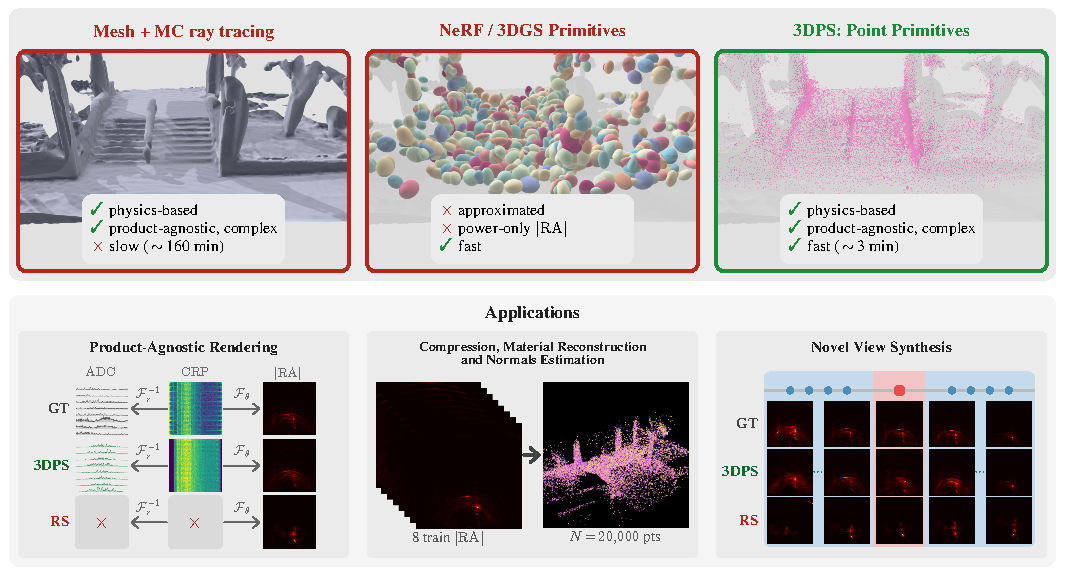
\includegraphics[width=\linewidth]{figs/teaser_3dps_v9b.pdf}
  \caption{\textbf{The right primitive for radar NVS.} Top: three method families on the three properties radar NVS demands (multi-viewpoint-tractable, physics-faithful, complex-valued). MC ray-tracing renderers (mmIR, Sionna RT) are physically faithful but too slow for multi-viewpoint optimization; optical-NVS adaptations (RadarSplat, Radar Fields, DART) are fast but discard phase. 3DPS is the first to satisfy all three. Bottom: 3DPS outputs on the held-out test frame of S1\,F185 --- $|\mathrm{RA}|$ render, raw ADC magnitude (inverse range FFT), and the optimized point cloud colored by learned $\varepsilon_r'$.}
  \label{fig:teaser}
\end{figure}

Millimeter-wave (mmWave) radar penetrates fog, rain, and airborne dust~\cite{guan2020through}, returns Doppler velocity directly, and is an essential sensor for robust perception in autonomous driving and robotics~\cite{gao2019experiments}. However, radar datasets are substantially smaller than their optical or LiDAR counterparts because radar sensors are not ubiquitous, the captured data structure depends heavily on array geometry and application-specific waveform configuration, and most large-scale datasets remain proprietary. NVS for radar can address this data scarcity by enabling sparse training sets to generalize across novel poses, but this problem is structurally hard. The supervision signal is typically i) sparse with returns dominated by quasi-mirror specular reflections at 60--77\,GHz, ii) constrained to 2D as COTS radar array geometries lack an elevation aperture and integrate out the elevation dimension, and iii) limited in view count as NVS aggregates only a handful of training views per scene.

Achieving high-fidelity radar NVS requires a renderer with three properties. First, multi-viewpoint-tractable, since NVS by definition demands joint optimization across many training poses. Second, physically faithful, so that predictions at unseen poses match the underlying sensor physics and the optimized scene parameters remain interpretable, editable, and transferable across sensor views. Third, complex-valued, since the radar forward model emits a complex phasor that is product-agnostic: the same optimized scene synthesizes raw analog-to-digital converter (ADC) samples, complex range profile (CRP), and range--azimuth (RA) outputs at novel viewpoints through standard FFT pipelines, without retraining (Fig.~\ref{fig:teaser}). We show that this also allows the renderer to reproduce antenna patterns, sidelobes, and FFT windowing from the signal model, sharpening RA correctness. Phase-discarding renderers forfeit both.

No prior method has all three properties. Differentiable Monte Carlo (MC) ray tracers~\cite{sionna, hofmann2025inverse, chen2025invertwin, mmIR2026} implement the radar forward model with explicit BSDF material modeling, real antenna beam patterns, and complex outputs. The cost is structural, since each surface hit must be evaluated against every (TX, RX) pair to maintain MIMO coherence. The closest prior work, mmIR~\cite{mmIR2026}, requires ${\sim}20$ minutes per single-viewpoint fit at 24k surface interactions, which does not scale to the multi-view optimization NVS demands. Optical-NVS adaptations~\cite{huang2024dart, 10.1145/3641519.3657510, takawale2025spinr, kung2025radarsplat} of neural radiance fields, hash grids, and 3D Gaussians~\cite{mildenhall2021nerf, 3dgs} train fast on real radar captures, because they trade explicit modeling of the radar signal chain for runtime. Supervision is on post-FFT power-only RA images, phase is dropped by construction, and the radar's signal-model components are absorbed into learned features rather than rendered.

3DPS realizes all three properties, because we derive it directly from the standard solid-angle form of the radar equation~\cite{skolnik2001introduction, mmIR2026}. For multi-viewpoint tractability, we splat each point's complex phasor into range bins through a precomputed Hann-windowed point spread function (PSF) at constant cost per (point, range bin), fuse BSDF evaluation and splatting into three CUDA kernels, and exploit a quasi-static MIMO factorization that linearizes the BSDF cost in $N_{\text{TX}} + N_{\text{RX}}$. For physical fidelity, the antenna geometry, BSDF (per ITU-R~P.2040), and antenna gains are evaluated in closed form with no learned features, and phase is integrated from the geometric path length rather than learned. For complex-valued output, the per-(TX, RX) range profile is preserved end-to-end through PSF splatting, enabling product-agnostic rendering to ADC, CRP, and RA without retraining via standard FFT pipelines.

We evaluate sparse-view radar NVS on six outdoor ColoRadar~\cite{kramer2022coloradar} scenes, measuring all three downstream products from the same optimized scene. On the held-out test view, 3DPS reaches \textbf{0.587} mean Pearson correlation on $|\mathrm{RA}|$, beating RadarSplat ($0.333$), Radar Fields ($0.120$), and DART ($0.081$) by $1.8\times$, $4.9\times$, and $7.2\times$ respectively. Further, 3DPS reaches \textbf{0.603} mean correlation on $|\mathrm{CRP}|$ and \textbf{0.613} on the ADC envelope. Training takes ${\sim}3$~minutes per scene on a single RTX~4090 across 8 training viewpoints jointly, ${\sim}50\times$ faster than the SOTA MC ray tracer's projected ${\sim}160$~min per-scene cost.

\textbf{Contributions.} \textbf{(i)} The first differentiable point renderer for radar, with a radar-native primitive (oriented 3D points carrying ITU-R~P.2040 material parameters) and multi-viewpoint-tractable rendering operation (PSF splatting of complex phasors into range bins), derived from the solid-angle form of the radar equation. \textbf{(ii)} Product-agnostic rendering, since the same optimized scene yields CRP, ADC, and RA outputs through standard FFT pipelines without retraining. \textbf{(iii)} Sparse-view radar NVS at the state of the art on $|\mathrm{RA}|$, $|\mathrm{CRP}|$, and ADC envelope across six ColoRadar scenes, ${\sim}50\times$ faster per scene than the SOTA MC ray tracer.
